\documentclass[tikz,border=8pt]{standalone}
% Shared look for every TikZ diagram. Load with \input{../../tools/tikz-style.tex}
\usepackage[T1]{fontenc}
\usepackage{lmodern}
\renewcommand{\sfdefault}{lmr}  % diagrams use the same serif as the text
\usetikzlibrary{arrows.meta, positioning, shapes.geometric, calc, fit, backgrounds}
\definecolor{cblue}{HTML}{4C78A8}
\definecolor{corange}{HTML}{F58518}
\definecolor{cgreen}{HTML}{54A24B}
\definecolor{cred}{HTML}{E45756}
\definecolor{cpurple}{HTML}{B279A2}
\definecolor{cgrey}{HTML}{6B6B6B}
\tikzset{
  every picture/.style={font=\sffamily, line width=1.2pt},
  box/.style={draw=#1, fill=#1!12, rounded corners=4pt, align=center, inner sep=7pt, minimum height=1.1cm},
  box/.default=cgrey,
  arrow/.style={-{Stealth[length=3mm]}, draw=cgrey, line width=1.4pt},
  title/.style={font=\sffamily\bfseries\Large},
  note/.style={font=\sffamily\small, text=cgrey, align=center},
}
\AtBeginDocument{\hyphenpenalty=10000 \exhyphenpenalty=10000}

\begin{document}
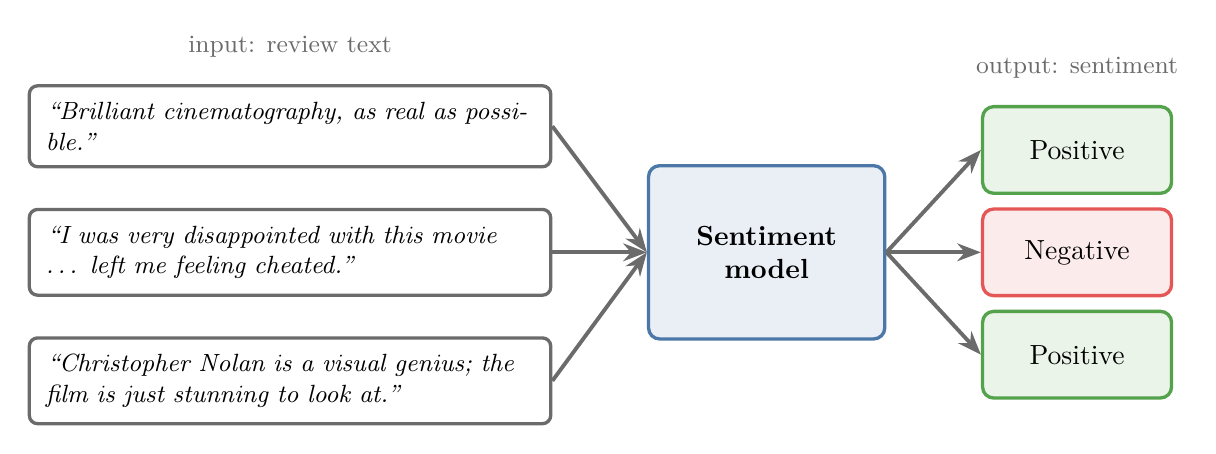
\begin{tikzpicture}[node distance=0.5cm and 1.2cm]
  \tikzset{rev/.style={draw=cgrey, fill=white, rounded corners=3pt, text width=6.2cm, align=left, inner sep=6pt, font=\small\itshape}}
  \node[rev] (r1) {``Brilliant cinematography, as real as possible.''};
  \node[rev, below=of r1] (r2) {``I was very disappointed with this movie \dots\ left me feeling cheated.''};
  \node[rev, below=of r2] (r3) {``Christopher Nolan is a visual genius; the film is just stunning to look at.''};
  \node[box=cblue, minimum width=3.0cm, minimum height=2.2cm, right=of r2] (m) {\textbf{Sentiment}\\\textbf{model}};
  \node[box=cgreen, right=of m, yshift=1.3cm, minimum width=2.4cm] (p1) {Positive};
  \node[box=cred, right=of m, minimum width=2.4cm] (n1) {Negative};
  \node[box=cgreen, right=of m, yshift=-1.3cm, minimum width=2.4cm] (p2) {Positive};
  \foreach \r in {r1,r2,r3} \draw[arrow] (\r.east) -- (m.west);
  \draw[arrow] (m.east) -- (p1.west);
  \draw[arrow] (m.east) -- (n1.west);
  \draw[arrow] (m.east) -- (p2.west);
  \node[note, above=0.2cm of r1] {input: review text};
  \node[note, above=0.2cm of p1] {output: sentiment};
\end{tikzpicture}
\end{document}
